\documentclass[a4paper,11pt]{refart}
\usepackage{listingsutf8}
\usepackage[brazilian]{babel}%Sinais e pountuação em portugês
\usepackage[utf8]{inputenc}
\usepackage[T1]{fontenc} % LY1 also works
\usepackage{tikz}
\usetikzlibrary{shapes,arrows}
%% Font settings suggested by fbb documentatio
\usepackage{float} 
\usepackage{listings}
\usepackage{microtype}
\usepackage{graphicx}
\usepackage{enumitem}
\setlist{leftmargin=*}
\lstset{basicstyle=\ttfamily,frame=single,xleftmargin=1em,xrightmargin=1em}
\usepackage[os=win]{menukeys}
\renewmenumacro{\keys}[+]{shadowedroundedkeys}
\usepackage{framed}
\usepackage{etoolbox}
\AtBeginEnvironment{leftbar}{\sffamily\small}
\usepackage[T1]{fontenc}
\usepackage{lmodern}
\usepackage{hyperref}
\usepackage{multirow}                                               
\usepackage{multicol}                                               
\usepackage{longtable}
\usepackage{amsmath}
\usepackage{dcolumn}
\usepackage{booktabs}
\usepackage{makecell}
\hyphenation{Trans-fe-rên-cias} %Hifenação de palavras

\hypersetup{colorlinks=true,linkcolor=black,citecolor=blue,urlcolor=blue}

\renewcommand\theadalign{bc}
\renewcommand\theadfont{\bfseries}
\renewcommand\theadgape{\Gape[4pt]}
\renewcommand\cellgape{\Gape[4pt]}


\def\CS#1{\texttt{\textbackslash#1}}

\usepackage[most]{tcolorbox}
\newtcblisting{commandshell}{colback=black,colupper=green,colframe=black!75!black,
	listing only,listing options={style=tcblatex,language=sh},
	every listing line={\textcolor{red}{\small\ttfamily\bfseries computer@user:\$ }}}

\usepackage[most]{tcolorbox}
\newtcblisting{shell}{colback=black,colupper=green,colframe=black!75!black,
	listing only,listing options={style=tcblatex,language=sh},
	every listing line={\textcolor{red}{\small\ttfamily\bfseries  }}}

\usepackage[most]{tcolorbox}
\newtcblisting{pymol}{colback=white,colupper=black,colframe=gray!75!black,
	listing only,listing options={style=tcblatex,language=sh},
	every listing line={\textcolor{red}{\small\ttfamily\bfseries  }}}



\title{ \huge {XI EMMSB }\\
		Instruções dos Tutoriais do PRIMoRDiA }
\author{Igor Barden Grillo \\(\url{barden.igor@gmail.com} )\\\url{github.com/bardenChem}}

\begin{document}
	\maketitle
	
	
	\hspace*{-1.2\leftmarginwidth}
	\begin{minipage}{\fullwidth}
		\begin{figure}[H]
			\begin{center}
				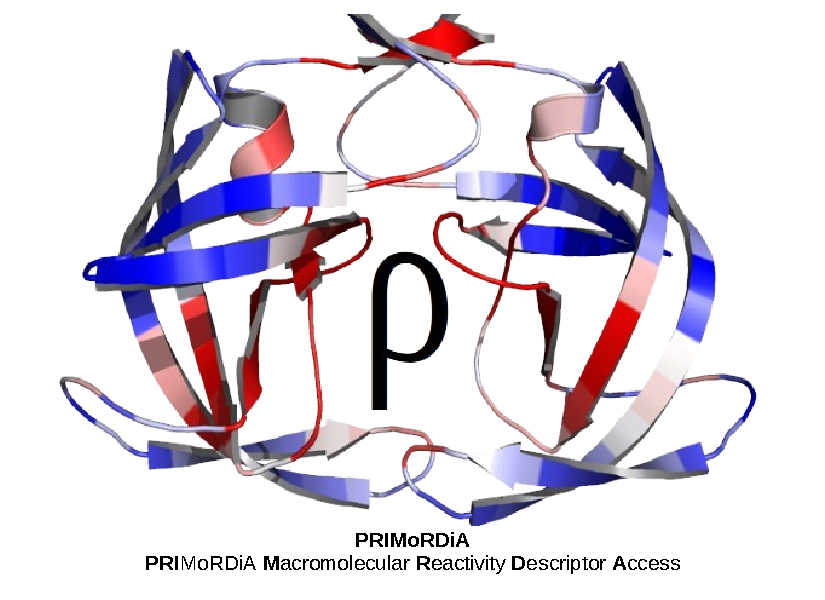
\includegraphics[width=7in]{logo_primordia}
			\end{center}
		\end{figure}	
	\end{minipage}	
	\newpage
	
	\newpage
	
	Esse documento tem como objetivo trazer todos os comandos e instruções diretas para a execução dos tutoriais ministrados no mini-curso na XI edição da Escola de Modelagem Molecular de Sistemas Biológicos (EMMSB) do Laboratório Nacional de Computação Científica (LNCC). Para a descrição completa dos tutoriais, material de referência e ilustração dos resultados esperados, confira o outro documento incluso nos materiais disponíveis desse mini-curso.
	
		
		
	\section{Tutorial 1: Complexos Proteína-Ligante}
	
	Nesse tutorial iremos:
	
	\begin{enumerate}
		\item Montar o input para os cálculos no PRIMoRDiA para os complexos RTA-Ligante
		\item Executar o PRIMoRDIA 
		\item Analisar os arquivos de saída
		\item Visualizar os mapas de reatividade no Pymol e salvar as imagens em alta resolução
	\end{enumerate}

	Primeiro comando:
	
	\hspace*{-\leftmarginwidth}
	\begin{minipage}{\fullwidth}
		\begin{commandshell}path/to/PRIMoRDiA_1.25v -input -op 3 -p mopac\end{commandshell}
	\end{minipage}

	Segundo Comando:
	
	\hspace*{-\leftmarginwidth}
	\begin{minipage}{\fullwidth}
		\begin{commandshell}path/to/PRIMoRDiA_1.25v -f primordia_editado.input\end{commandshell}
	\end{minipage}

	Para a análise dos resultados no Pymol, vamos primeiro abrir o software e executar o comando 
	
	\hspace*{-\leftmarginwidth}
	\begin{minipage}{\fullwidth}
		\begin{pymol}@19m_pymols_pdb.pym\end{pymol}
	\end{minipage}
	
	Vamos ativar o objeto "netphilicity" e executar o seguinte comando no Pymol 
	
	 \hspace*{-\leftmarginwidth}
	 \begin{minipage}{\fullwidth}
	 	\begin{pymol}spectrum b, blue_white_red, minimum=-0.1,maximum=0.1\end{pymol}
	 \end{minipage}
	
	Depois vamos ativar o objeto "hardness\_fukui\_pot\_left" e executar o comando


	\hspace*{-\leftmarginwidth}
	\begin{minipage}{\fullwidth}
		\begin{pymol}spectrum b, white_yellow_orange_red_black, minimum=-0.1,maximum=0.25\end{pymol}
	\end{minipage}
	
	E depois ajustar o comando para
	
	\hspace*{-\leftmarginwidth}
	\begin{minipage}{\fullwidth}
		\begin{pymol}spectrum b, white_yellow_orange_red_black, minimum=-0.15,maximum=0.23\end{pymol}
	\end{minipage}

	Ajustar o tipo de tracejado ao redor da molécula 
	
	
	\hspace*{-\leftmarginwidth}
	\begin{minipage}{\fullwidth}
		\begin{pymol}set ray_trace_mode, 1\end{pymol}
	\end{minipage}

	Renderizar a molécula em alta qualidade

	\hspace*{-\leftmarginwidth}
	\begin{minipage}{\fullwidth}
		\begin{pymol}ray antialias=2\end{pymol}
	\end{minipage}

	E salvar 
	
	\hspace*{-\leftmarginwidth}
	\begin{minipage}{\fullwidth}
		\begin{pymol}png complex_rta_19m_hardness.png\end{pymol}
	\end{minipage}

	
	\section{Tutorial 2: Gerando Trajetória de Catálise Enzimática} 
	
	Com todos os programas devidamente instalados, nesse tutorial, vamos executar um script em Pyhton já fornecido no material do mini-curso, a realizar a análise dos resultados. Durante o mini-curso, vamos avaliar como foi montado esse script em Python para que se de uma noção de como pode ser montado para outros sistemas e simulações. 
	
	Dentro da pasta do mini-curso, no diretório Reaction, já se encontram os arquivos de campo de força e coordenadas do sistema enzimático de teste, o script em Python e algumas etapas já prontas, pois são demoradas. O único comando a ser executado será: 
	
	\hspace*{-\leftmarginwidth}
	\begin{minipage}{\fullwidth}
		\begin{commandshell}python3 Reaction_TIM.py\end{commandshell}
	\end{minipage}
	
	Outras atividades serão: abrir os gráficos de energia versus coordenada de reação, e visualizar o caminho de reação no Pymol. 
	
	\section{Tutorial 3: Análise de Reatividade de Caminho de Reação Enzimático} 
	
	Nesse tutorial vamos executar o PRIMoRDiA em um modo diferente, que trata arquivos de estrutura eletrônica que estejam relacionados entre si por ordem de Frames, ou seja uma trajetória. Vamos usar os arquivos ".aux" do método RM1 calculado no refinamento de energia no mopac, mas primeiro, é necessário mudar o nome desses arquivos, tirando o "rm1", do nome para que o PRIMoRDiA reconheça a sequência dos frames pela extensão do arquivo. Isso pode ser realizado facilmente com essas linhas de comando no terminal.
	
		\hspace*{-\leftmarginwidth}
	\begin{minipage}{\fullwidth}
		\begin{commandshell}for file in *rm1.aux; 
			do 
			mv "$file" "${file/_rm1.aux/.aux}";
			done	\end{commandshell}
	\end{minipage}
	
	\hspace*{-\leftmarginwidth}
	\begin{minipage}{\fullwidth}
		\begin{commandshell}for file in *rm1.pdb; 
			do 
			mv "$file" "${file/_rm1.pdb/.pdb}";
			done\end{commandshell}
	\end{minipage}

	 O input para esse tutorial pode ser copiado e colado em um editor de texto a partir dos dados fornecidos na próxima caixa de texto
	 
	 	 \hspace*{-\leftmarginwidth}
	 \begin{minipage}{\fullwidth}
	 	\begin{lstlisting}[caption={Input editado para execução do tutorial 3},label={tut402}]
#RT reaction 
#PR eband 3 Rscript pymols
#Reaction RC1 137 138 73
#Reaction dimX 20
#TRJ residues 3 4 9
3 frame.aux true 30 10 frame.pdb mopac  0 0 0 0 EW
	 	\end{lstlisting}
	 \end{minipage}
	 
	Salve esse arquivo na pasta onde os arquivos de estrutura eletrônica ficaram salvos, e rode com o seguinte comando 
	
	\hspace*{-\leftmarginwidth}
	\begin{minipage}{\fullwidth}
		\begin{commandshell}path/to/PRIMoRDiA_1.25v -f reaction_analysis.input\end{commandshell}
	\end{minipage}

	Para gerar os gráficos de variação dos descritores globais e para os átomos da coordenada de reação usando o R, vamos rodar o comando abaixo
	
	
	\hspace*{-\leftmarginwidth}
	\begin{minipage}{\fullwidth}
		\begin{commandshell}Rscript frame0_reaction_analysis.R\end{commandshell}
	\end{minipage}

	Depois de análisar esses gráficos, vamos gerar algumas visualizações dos descritores volumétricos no Pymol. Só abrir o programa e executar o seguinte comando
	
	
 	\hspace*{-\leftmarginwidth}
	\begin{minipage}{\fullwidth}\begin{pymol}@frame0_pymols.pym\end{pymol}
	\end{minipage}
	
	Vamos explorar as visualizações volumétricas e aprender a renderizar e salvar as imagens. 
	
	Para os descritores condensados, vamos abrir a estrutura inicial e a estrutura do estado de transição com os seguintes comando no Pymol 
	
	\hspace*{-\leftmarginwidth}
	\begin{minipage}{\fullwidth}\begin{pymol}@frame0_pymols_pdb.pym\end{pymol}
	\end{minipage}


	\hspace*{-\leftmarginwidth}
	\begin{minipage}{\fullwidth}\begin{pymol}@frame15_pymols_pdb.pym\end{pymol}
	\end{minipage}

	Para finalizar as análises, vamos utilizar o R novamente para gerar gráficos com as estatísticas dos descritores para os resíduos e substrato durante a trajetória, com o seguinte comando 

	\hspace*{-\leftmarginwidth}
	\begin{minipage}{\fullwidth}
		\begin{commandshell}Rscript frame0_reaction_analysis.R\end{commandshell}
	\end{minipage}
	
	\section{Instalação dos Programas}
	
	A maioria dos softwares já estarão instalados nos computadores do mini-curso. Para alguns deles, nós veremos durante o tutorial como configurar variável de caminho e outras opções. No entanto, as instruções da instalação dos  programas citados nesses tutoriais  estão logo abaixo. Informações mais específicas sobre compilação, instalação e uso dos binários já compilados, consulte o guia de usuário fornecido no repositório. 
	
	\subsection{PRIMoRDiA Software}
	
	Para baixar os dados do repositório é possível usar o seguinte comando do git:
	
\hspace*{-\leftmarginwidth}
\begin{minipage}{\fullwidth}
\begin{commandshell}git clone https://github.com/igorChem/PRIMoRDiA1.0v.git\end{commandshell}
\end{minipage}
	
	Por padrão, o PRIMoRDiA utiliza o g++ e a biblioteca Eigen 3. Para assegurar que sua máquina tenha o necessário para compilar o PRIMoRDiA, execute os comandos abaixo
	
\hspace*{-\leftmarginwidth}
\begin{minipage}{\fullwidth}
\begin{commandshell}sudo apt install g++
sudo apt install cmake	
sudo apt install libeigen3-dev
\end{commandshell}
\end{minipage}

	Depois de descomprimir a pasta baixada com a versão estável, entre no diretório e faça a compilação usando os seguintes comandos: 
	
\hspace*{-\leftmarginwidth}
\begin{minipage}{\fullwidth}
\begin{commandshell}cd /caminho/da/pasta/PRIMoRDiA1.0v
cmake .
make
\end{commandshell}
\end{minipage}
	
	O processo de compilação deve ocorrer sem problemas e gerar um arquivo binário chamado "PRIMoRDIA\_1.25v\_LINUX64 ", caso a versão 1.25 seja a escolhida ( mais recomendado ).
	Com o comando descrito abaixo é possível criar um atalho para executar o programa de qualquer diretório do seu sistema
	
	\subsection{Pymol} 
	
	Nos ambientes linux baseados em Debian, isto é, que utilizam o sistema apt-get para a instalação dos pacotes pelo repositório, o Pymol apresenta um versão padrão em condições satisfatórias para uso geral e para as virtualizações requeridas nesses tutoriais. Portanto, com o seguinte comando é possível instalar o programa
	
	\hspace*{-\leftmarginwidth}
	\begin{minipage}{\fullwidth}
		\begin{commandshell}sudo apt-get install pymol\end{commandshell}
	\end{minipage}
	
	\subsection{pDynamo}
	
	Para instalar o pDynamo primeiro baixe ou clone o repositório do Git Hub, que pode ser feito com o seguinte comando
	
	
\hspace*{-\leftmarginwidth}
\begin{minipage}{\fullwidth}
\begin{commandshell}git clone https://github.com/pdynamo/pDynamo3.git\end{commandshell}
\end{minipage}	

	Para a instalação é necessário conferir a existência de algumas bibliotecas, compiladores e módulos instalados no Python: Python 3, versão 3.5 ou mais atualizada; Cython, instala o compilador e o módulo pelo pip 
	
\hspace*{-\leftmarginwidth}
\begin{minipage}{\fullwidth}
\begin{commandshell}sudo apt-get install cython3\end{commandshell}
\begin{commandshell}pip install cython\end{commandshell}
\end{minipage}



	PyMal
	
\hspace*{-\leftmarginwidth}
\begin{minipage}{\fullwidth}
	\begin{commandshell}sudo apt-get install python3-yaml\end{commandshell}
\end{minipage}	

	E um compilador de C, mas para usar o PRIMoRDIA, o compilador do GCC já se instalou quando o g++ foi instalado. A instalação do pDynamo se dá no diretório "installation", com o seguinte comando
	

\hspace*{-\leftmarginwidth}
\begin{minipage}{\fullwidth}
	\begin{commandshell}python3 Install.py -f\end{commandshell}
\end{minipage}

	Para o programa funcionar ele precisa ter suas biblioteca no caminho do Python e a configurar de outras variáveis. Para isso, abra o arquivo ".bashrc", localizado no seu diretório "/home/usuário" e adicionar as linhas (não esqueça de editar elas antes)
	
\hspace*{-\leftmarginwidth}
\begin{minipage}{\fullwidth}
\begin{shell}PDYNAMO3_HOME=/home/usuário/programs/pDynamo3;export PDYNAMO3_HOME
export PDYNAMO3_PARAMETERS=$PDYNAMO3_HOME/parameters  
export PDYNAMO3_PYTHONCOMMAND=python3
export PDYNAMO3_SCRATCH=$PDYNAMO3_HOME/scratch 
export PDYNAMO3_STYLE=$PDYNAMO3_PARAMETERS/ccsStyleSheets/defaultStyle.css
export PYTHONPATH=$PDYNAMO3_HOME:$PYTHONPATH
\end{shell}
\end{minipage}	
	
	\subsection{pDynamo\_Scripts}
	
	
	A "instalação" do pDynamo\_scripts se dá pelo download do repositório do Git Hub, que pode ser feito apenas clonando o repositório com o comando mostrado a baixo
	
	\hspace*{-\leftmarginwidth}
	\begin{minipage}{\fullwidth}
		\begin{commandshell}git clone https://github.com/bardenChem/pDynamo3_scripts.git\end{commandshell}
	\end{minipage}
	
	Para ativar o pDynamo3 e  pDynamo\_scripts é necessário colocar os scripts no caminho de execução de bibliotecas do Python3, o que foi deixado para esse tutorial, pois é algo que as vezes causa confusão. Abra o arquivo ".bashrc" e adione a seguinte linha. 
	
	\hspace*{-\leftmarginwidth}
	\begin{minipage}{\fullwidth}
		\begin{commandshell}export PYTHONPATH=$HOME/pDynamo3_scripts:$PYTHONPATH\end{commandshell}
	\end{minipage}
	
	O pDynamo\_scripts ainda está em desenvolvimento, mas diversas funcionalidades já estão disponíveis e podem ser conferidas nos arquivos da pasta de teste, que tem um modelo básico para rodar diversos tipos de simulação.
	

\end{document}